%! Author = Omar Iskandarani
%! Title = Emergent General Relativity from Structured Swirl Dynamics in the Vortex Æther Model (VAM)
%! Date = 21-06-2025
%! Affiliation = Independent Researcher, Groningen, The Netherlands
%! License = © 2025 Omar Iskandarani. All rights reserved. This manuscript is made available for academic reading and citation only. No republication, redistribution, or derivative works are permitted without explicit written permission from the author. Contact: info@omariskandarani.com
%! ORCID = 0009-0006-1686-3961
%! DOI = 10.5281/zenodo.15712578

% === Metadata ===
\newcommand{\papertitle}{Emergent General Relativity from Structured Swirl Dynamics in the Vortex Æther Model (VAM)}
\newcommand{\paperdoi}{10.5281/zenodo.15712578}


\ifdefined\standalonechapter\else
% Standalone mode
\documentclass[12pt]{article}
\usepackage{tikz}
\usepackage{amsmath}
\usepackage[margin=1in]{geometry}
\usepackage[utf8]{inputenc}
\usepackage[T1]{fontenc}
\usepackage{amssymb}
\usepackage{hyperref}
\usetikzlibrary{arrows.meta, positioning, shapes.multipart}
\usepackage{amsthm}
\newtheorem{theorem}{Theorem}[section]
\newtheorem{lemma}[theorem]{Lemma}
\usepackage{booktabs}
\usepackage{array}
\usepackage{bm}




% vamstyle.sty
\NeedsTeXFormat{LaTeX2e}
\ProvidesPackage{vamstyle}[2025/07/01 VAM unified style]

% === Constants ===
\newcommand{\hbarVal}{\ensuremath{1.054571817 \times 10^{-34}}} % J\cdot s
\newcommand{\meVal}{\ensuremath{9.10938356 \times 10^{-31}}} % kg
\newcommand{\cVal}{\ensuremath{2.99792458 \times 10^{8}}} % m/s
\newcommand{\alphaVal}{\ensuremath{1 / 137.035999084}} % unitless
\newcommand{\alphaGVal}{\ensuremath{1.75180000 \times 10^{-45}}} % unitless
\newcommand{\reVal}{\ensuremath{2.8179403227 \times 10^{-15}}} % m
\newcommand{\rcVal}{\ensuremath{1.40897017 \times 10^{-15}}} % m
\newcommand{\vacrho}{\ensuremath{5 \times 10^{-9}}} % kg/m^3
\newcommand{\LpVal}{\ensuremath{1.61625500 \times 10^{-35}}} % m
\newcommand{\MpVal}{\ensuremath{2.17643400 \times 10^{-8}}} % kg
\newcommand{\tpVal}{\ensuremath{5.39124700 \times 10^{-44}}} % s
\newcommand{\TpVal}{\ensuremath{1.41678400 \times 10^{32}}} % K
\newcommand{\qpVal}{\ensuremath{1.87554596 \times 10^{-18}}} % C
\newcommand{\EpVal}{\ensuremath{1.95600000 \times 10^{9}}} % J
\newcommand{\eVal}{\ensuremath{1.60217663 \times 10^{-19}}} % C

% === VAM/\ae ther Specific ===
\newcommand{\CeVal}{\ensuremath{1.09384563 \times 10^{6}}} % m/s
\newcommand{\FmaxVal}{\ensuremath{29.0535070}} % N
\newcommand{\FmaxGRVal}{\ensuremath{3.02563891 \times 10^{43}}} % N
\newcommand{\gammaVal}{\ensuremath{0.005901}} % unitless
\newcommand{\GVal}{\ensuremath{6.67430000 \times 10^{-11}}} % m^3/kg/s^2
\newcommand{\hVal}{\ensuremath{6.62607015 \times 10^{-34}}} % J Hz^-1

% === Electromagnetic ===
\newcommand{\muZeroVal}{\ensuremath{1.25663706 \times 10^{-6}}}
\newcommand{\epsilonZeroVal}{\ensuremath{8.85418782 \times 10^{-12}}}
\newcommand{\ZzeroVal}{\ensuremath{3.76730313 \times 10^{2}}}

% === Atomic & Thermodynamic ===
\newcommand{\RinfVal}{\ensuremath{1.09737316 \times 10^{7}}}
\newcommand{\aZeroVal}{\ensuremath{5.29177211 \times 10^{-11}}}
\newcommand{\MeVal}{\ensuremath{9.10938370 \times 10^{-31}}}
\newcommand{\MprotonVal}{\ensuremath{1.67262192 \times 10^{-27}}}
\newcommand{\MneutronVal}{\ensuremath{1.67492750 \times 10^{-27}}}
\newcommand{\kBVal}{\ensuremath{1.38064900 \times 10^{-23}}}
\newcommand{\RVal}{\ensuremath{8.31446262}}

% === Compton, Quantum, Radiation ===
\newcommand{\fCVal}{\ensuremath{1.23558996 \times 10^{20}}}
\newcommand{\OmegaCVal}{\ensuremath{7.76344071 \times 10^{20}}}
\newcommand{\lambdaCVal}{\ensuremath{2.42631024 \times 10^{-12}}}
\newcommand{\PhiZeroVal}{\ensuremath{2.06783385 \times 10^{-15}}}
\newcommand{\phiVal}{\ensuremath{1.61803399}}
\newcommand{\eVVal}{\ensuremath{1.60217663 \times 10^{-19}}}
\newcommand{\GFVal}{\ensuremath{1.16637870 \times 10^{-5}}}
\newcommand{\lambdaProtonVal}{\ensuremath{1.32140986 \times 10^{-15}}}
\newcommand{\ERinfVal}{\ensuremath{2.17987236 \times 10^{-18}}}
\newcommand{\fRinfVal}{\ensuremath{3.28984196 \times 10^{15}}}
\newcommand{\sigmaSBVal}{\ensuremath{5.67037442 \times 10^{-8}}}
\newcommand{\WienVal}{\ensuremath{2.89777196 \times 10^{-3}}}
\newcommand{\kEVal}{\ensuremath{8.98755179 \times 10^{9}}}

% === \ae ther Densities ===
\newcommand{\rhoMass}{\rho_\text{\ae}^{(\text{mass})}}
\newcommand{\rhoMassVal}{\ensuremath{3.89343583 \times 10^{18}}}
\newcommand{\rhoEnergy}{\rho_\text{\ae}^{(\text{energy})}}
\newcommand{\rhoEnergyVal}{\ensuremath{3.49924562 \times 10^{35}}}
\newcommand{\rhoFluid}{\rho_\text{\ae}^{(\text{fluid})}}
\newcommand{\rhoFluidVal}{\ensuremath{7.00000000 \times 10^{-7}}}

% === Draft Options ===
\newif\ifvamdraft
% \vamdrafttrue
\ifvamdraft
\RequirePackage{showframe}
\fi

% === Load Once ===
\RequirePackage{ifthen}
\newboolean{vamstyleloaded}
\ifthenelse{\boolean{vamstyleloaded}}{}{\setboolean{vamstyleloaded}{true}

% === Page ===
\RequirePackage[a4paper, margin=2.5cm]{geometry}

% === Fonts ===
\RequirePackage[T1]{fontenc}
\RequirePackage[utf8]{inputenc}
\RequirePackage[english]{babel}
\RequirePackage{textgreek}
\RequirePackage{mathpazo}
\RequirePackage[scaled=0.95]{inconsolata}
\RequirePackage{helvet}

% === Math ===
\RequirePackage{amsmath, amssymb, mathrsfs, physics}
\RequirePackage{siunitx}
\sisetup{per-mode=symbol}

% === Tables ===
\RequirePackage{graphicx, float, booktabs}
\RequirePackage{array, tabularx, multirow, makecell}
\newcolumntype{Y}{>{\centering\arraybackslash}X}
\newenvironment{tighttable}[1][]{\begin{table}[H]\centering\renewcommand{\arraystretch}{1.3}\begin{tabularx}{\textwidth}{#1}}{\end{tabularx}\end{table}}
\RequirePackage{etoolbox}
\newcommand{\fitbox}[2][\linewidth]{\makebox[#1]{\resizebox{#1}{!}{#2}}}

% === Graphics ===
\RequirePackage{tikz}
\usetikzlibrary{3d, calc, arrows.meta, positioning}
\RequirePackage{pgfplots}
\pgfplotsset{compat=1.18}
\RequirePackage{xcolor}

% === Code ===
\RequirePackage{listings}
\lstset{basicstyle=\ttfamily\footnotesize, breaklines=true}

% === Theorems ===
\newtheorem{theorem}{Theorem}[section]
\newtheorem{lemma}[theorem]{Lemma}

% === TOC ===
\RequirePackage{tocloft}
\setcounter{tocdepth}{2}
\renewcommand{\cftsecfont}{\bfseries}
\renewcommand{\cftsubsecfont}{\itshape}
\renewcommand{\cftsecleader}{\cftdotfill{.}}
\renewcommand{\contentsname}{\centering \Huge\textbf{Contents}}

% === Sections ===
\RequirePackage{sectsty}
\sectionfont{\Large\bfseries\sffamily}
\subsectionfont{\large\bfseries\sffamily}

% === Bibliography ===
\RequirePackage[numbers]{natbib}

% === Links ===
\RequirePackage{hyperref}
\hypersetup{
    colorlinks=true,
    linkcolor=blue,
    citecolor=blue,
    urlcolor=blue,
    pdftitle={The Vortex \AE ther Model},
    pdfauthor={Omar Iskandarani},
    pdfkeywords={vorticity, gravity, \ae ther, fluid dynamics, time dilation, VAM}
}
\urlstyle{same}
\RequirePackage{bookmark}

% === Misc ===
\RequirePackage[none]{hyphenat}
\sloppy
\RequirePackage{empheq}
\RequirePackage[most]{tcolorbox}
\newtcolorbox{eqbox}{colback=blue!5!white, colframe=blue!75!black, boxrule=0.6pt, arc=4pt, left=6pt, right=6pt, top=4pt, bottom=4pt}
\RequirePackage{titling}
\RequirePackage{amsfonts}
\RequirePackage{titlesec}
\RequirePackage{enumitem}

\AtBeginDocument{\RenewCommandCopy\qty\SI}

\pretitle{\begin{center}\LARGE\bfseries}
\posttitle{\par\end{center}\vskip 0.5em}
\preauthor{\begin{center}\large}
\postauthor{\end{center}}
\predate{\begin{center}\small}
\postdate{\end{center}}

\endinput
}
% vamappendixsetup.sty

\newcommand{\titlepageOpen}{
  \begin{titlepage}
  \thispagestyle{empty}
  \centering
  {\Huge\bfseries \papertitle \par}
  \vspace{1cm}
  {\Large\itshape\textbf{Omar Iskandarani}\textsuperscript{\textbf{*}} \par}
  \vspace{0.5cm}
  {\large \today \par}
  \vspace{0.5cm}
}

% here comes abstract
\newcommand{\titlepageClose}{
  \vfill
  \null
  \begin{picture}(0,0)
  % Adjust position: (x,y) = (left, bottom)
  \put(-200,-40){  % Shift 75pt left, 40pt down
    \begin{minipage}[b]{0.7\textwidth}
    \footnotesize % One step bigger than \tiny
    \renewcommand{\arraystretch}{1.0}
    \noindent\rule{\textwidth}{0.4pt} \\[0.5em]  % ← horizontal line
    \textsuperscript{\textbf{*}}Independent Researcher, Groningen, The Netherlands \\
    Email: \texttt{info@omariskandarani.com} \\
    ORCID: \texttt{\href{https://orcid.org/0009-0006-1686-3961}{0009-0006-1686-3961}} \\
    DOI: \href{https://doi.org/\paperdoi}{\paperdoi} \\
    License: CC-BY 4.0 International \\
    \end{minipage}
  }
  \end{picture}
  \end{titlepage}
}
\begin{document}

    % === Title page ===
    \titlepageOpen


    \begin{abstract}
        We present a unified derivation showing that both Special and General Relativity emerge as effective limiting behaviors of the Vortex Æther Model (VAM), a fluid-dynamic theory with absolute time and Euclidean space. In the low-vorticity limit, we formally recover the Lorentz-invariant observables of Special Relativity—time dilation, length contraction, and invariant intervals—as consequences of swirl field kinematics, establishing the Lorentz Recovery Theorem. Extending to curved swirl topologies, we demonstrate that key gravitational phenomena of General Relativity—including redshift, light deflection, and geodesic motion—arise from structured vorticity and pressure gradients in a compressible, inviscid æther. This suggests that spacetime curvature is not fundamental, but an emergent epiphenomenon of coherent vortex dynamics in a deeper fluid substratum.
    \end{abstract}

    \begin{figure}[h]
        \centering
        \small
        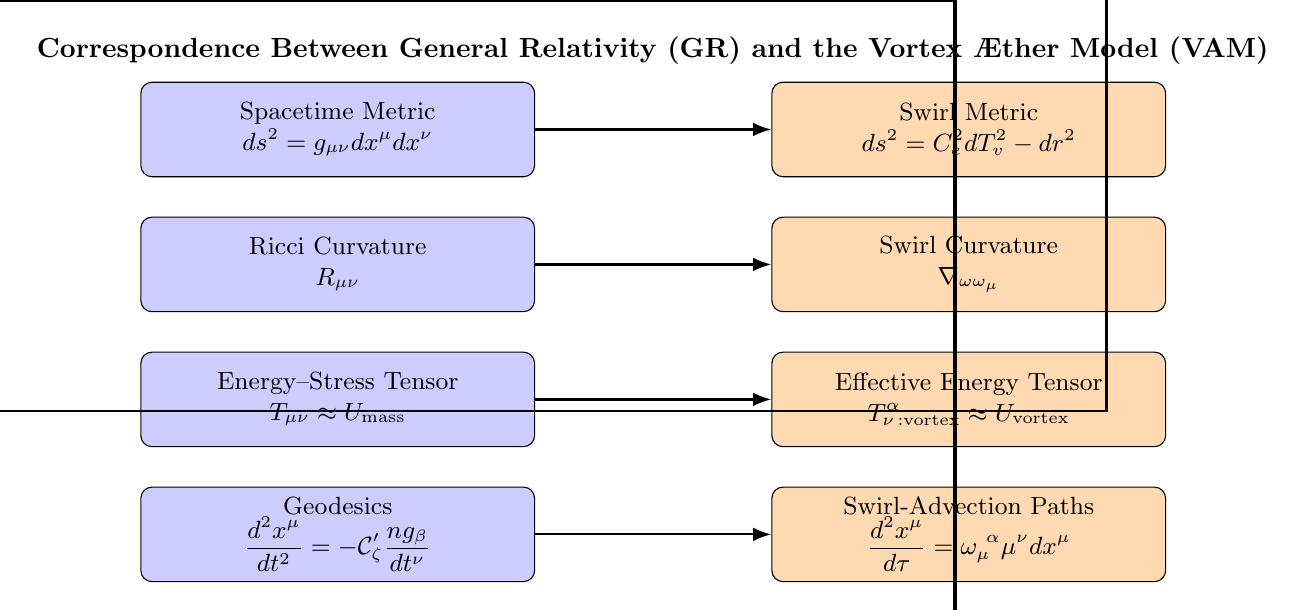
\begin{tikzpicture}[
            box/.style={rectangle, draw=black, rounded corners, minimum width=5cm, minimum height=1.2cm, text centered, font=\small},
            grbox/.style={box, fill=blue!20},
            vambox/.style={box, fill=orange!30},
            arrow/.style={-Latex, thick},
            node distance=0.5cm,
            every node/.append style={align=center}
        ]

% Left GR column (aligned)
            \node[grbox] (gr1) at (-4,4) {Spacetime Metric\\$ds^2 = g_{\mu\nu} dx^\mu dx^\nu$};
            \node[grbox, below=of gr1] (gr2) {Ricci Curvature\\$R_{\mu\nu}$};
            \node[grbox, below=of gr2] (gr3) {Energy–Stress Tensor\\$T_{\mu\nu} \approx U_{\text{mass}}$};
            \node[grbox, below=of gr3] (gr4) {Geodesics\\$\displaystyle\frac{d^2 x^\mu}{dt^2} = -\mathcal{C}'_\zeta \frac{n g_\beta}{dt^\nu}$};

% Right VAM column
            \node[vambox, right=3cm of gr1] (vam1) {Swirl Metric\\$ds^2 = C_e^2 dT_v^2 - dr^2$};
            \node[vambox, below=of vam1] (vam2) {Swirl Curvature\\$\nabla_{\omega\omega_\mu}$};
            \node[vambox, below=of vam2] (vam3) {Effective Energy Tensor\\$T^\alpha_{\nu\,:\text{vortex}} \approx U_{\text{vortex}}$};
            \node[vambox, below=of vam3] (vam4) {Swirl-Advection Paths\\$\displaystyle\frac{d^2 x^\mu}{d\tau} = \omega_\mu^{\ \alpha} \mu^\nu dx^\mu$};

% Horizontal arrows
            \draw[arrow] (gr1.east) -- (vam1.west);
            \draw[arrow] (gr2.east) -- (vam2.west);
            \draw[arrow] (gr3.east) -- (vam3.west);
            \draw[arrow] (gr4.east) -- (vam4.west);

% Title
            \node at (0,5) {\textbf{Correspondence Between General Relativity (GR) and the Vortex Æther Model (VAM)}};

        \end{tikzpicture}
        \caption{Side-by-side correspondence between General Relativity and the Vortex Æther Model.}
        \label{fig:gr-vam-centered}
    \end{figure}

    \titlepageClose
    \fi

    \ifdefined\standalonechapter
    \section{\papertitle}
    \else
    \fi
% ============= Begin of content ============
\section*{Lorentz Recovery Theorem in the Vortex Æther Model}

    \subsection*{Core Postulates of the Vortex Æther Model (VAM)}

    \begin{description}
        \item[\textbf{1. Aithēr-Time \(\mathcal{N}\)}]%
        The universal time coordinate \( \mathcal{N} \in \mathbb{R} \) flows uniformly and globally throughout the æther. It defines a shared causal substrate and temporal ordering of all events. (See Appendix~\ref{sec:temporal-constructs}.)

        \item[\textbf{2. Euclidean Æther Space}]%
        Physical space is flat \( \mathbb{R}^3 \), with a preferred æther rest frame \( \Xi_0 \). The æther medium is modeled as an inviscid, approximately incompressible, superfluid-like continuum with background density \( \rho_{\text{\ae}} \).

        \item[\textbf{3. Swirl Field Dynamics}]%
        Vortical excitations are governed by tangential velocity \( \vec{v}_\theta = \vec{\omega} \times \vec{r} \), where \( \vec{\omega} \) is local angular velocity. Circulation is quantized and conserved along vortex filaments.

        \item[\textbf{4. Knotted Particles}]%
        Stable matter is realized as topologically knotted or closed-loop vortex structures embedded in the æther. Persistence arises from conserved topology and internal swirl invariants.

        \item[\textbf{5. Time Dilation from Vortex Motion}]%
        The proper time \( \tau \) experienced by a vortex relates to universal time \( \mathcal{N} \) by:
        \begin{equation}
            \boxed{
                \frac{d\tau}{d\mathcal{N}} = \sqrt{1 - \frac{|\vec{v}_\theta|^2}{c^2}}, \quad |\vec{v}_\theta| = |\vec{\omega}| r
            }
            \label{eq:tau-dilation}
        \end{equation}


        \item[\textbf{6. Local Temporal Modes}]%
        Vortices carry internal clocks, including:
        \begin{itemize}
            \item Proper time \( \tau \)
            \item Swirl phase clock \( S(t)^{\circlearrowleft\!/\!\circlearrowright} \)
            \item Vortex proper time \( T_v = \oint \frac{ds}{v_\text{phase}} \)
        \end{itemize}
        All desynchronize relative to \( \mathcal{N} \) in high-swirl or pressure regions.

        \item[\textbf{7. Gravity from Swirl Pressure}]%
        Gravitational phenomena (time dilation, lensing, geodesics) arise from nonlinear swirl-induced pressure gradients. Spacetime curvature is emergent, not fundamental.
    \end{description}

% -------------------------------------------------

    \subsection*{Key Definitions}

    \begin{description}

        \item[\textbf{Swirl Energy Density}]%
        \[
            U_{\text{vortex}} = \frac{1}{2} \rho_{\text{\ae}}^{\text{(energy)}} |\vec{\omega}|^2.
        \]
        Represents localized rotational energy density. Serves as the source of inertial and gravitational-like effects in VAM, analogous to energy-momentum in GR.

        \item[\textbf{Swirl Clock Phase Gradient}]%

        \begin{equation}
            \boxed{
                \nabla S(t) = \frac{dS}{d\mathcal{N}} + \vec{\omega}(\tau) \cdot \hat{n}
            }
            \label{eq:swirl-clock-gradient}
        \end{equation}

        where \( \hat{n} \) is the unit vector along the knot’s internal clock axis. Describes local phase evolution, rotation, and chirality state.

        \item[\textbf{Vortex Proper Time \( T_v \)}]%

        \begin{equation}
            \boxed{
                T_v = \oint \frac{ds}{v_\text{phase}}
            }
            \label{eq:vortex-proper-time}
        \end{equation}

        Time internal to a closed-loop vortex. Tracks periodicity, identity, and quantum-like behavior from fluid topology.
    \end{description}

% -------------------------------------------------

    \begin{tcolorbox}[title=Key Temporal Variables in VAM]
        \begin{itemize}
            \item \( \mathcal{N} \) — Aithēr-Time (absolute, global)
            \item \( \tau \) — Chronos-time (proper, local)
            \item \( S(t)^{\circlearrowleft/\circlearrowright} \) — Swirl Clock (internal, cyclical)
            \item \( T_v = \oint \frac{ds}{v_{\text{phase}}} \) — Vortex Proper Time (loop-based, topological)
        \end{itemize}
        Each represents a different slicing or rhythm of time under the Vortex Æther ontology.
    \end{tcolorbox}

% -------------------------------------------------

    \subsection*{Lemmas}

    \begin{lemma*}[Emergent Time Dilation]
        For a vortex with rigid swirl speed \( v = |\vec{\omega}| r \), the time dilation obeys equation ~\eqref{eq:tau-dilation}. This mirrors the Lorentz factor from special relativity.
    \end{lemma*}

    \begin{lemma*}[Length Contraction from Swirl Pressure]
        Front-back asymmetry in translating vortices yields phase compression:
        \begin{equation}
            \boxed{
                L = L_0 \sqrt{1 - \frac{v^2}{c^2}}.
            }
            \label{eq:lorentz-length-contraction}
        \end{equation}
        This mirrors the Lorentz contraction in special relativity, where \( L_0 \) is the proper length.
    \end{lemma*}

    \begin{lemma*}[Invariant Interval from Swirl Metric]
        Let:
        \begin{equation}
            \boxed{
                ds^2 = C_e^2 dT_v^2 - dr^2
            }
            \label{eq:swirl-metric}
        \end{equation}
        Then in the limit \( \omega \to 0 \), \( T_v \to \tau \) and:
        \[
            ds^2 \to c^2 d\tau^2 - dr^2.
        \]
    \end{lemma*}

% -------------------------------------------------

    \subsection*{Theorem (Lorentz Recovery Theorem)}

    \begin{theorem*}[Lorentz Recovery Theorem]
        Let a vortex structure propagate through the æther with tangential swirl velocity \( |\vec{v}_\theta| \ll c \). Then the Vortex Æther Model (VAM) reproduces all first-order Lorentz-invariant observables of special relativity:

        \begin{itemize}
            \item \textbf{Time Dilation:} \( \tau = \mathcal{N} / \gamma(v) \)
            \item \textbf{Length Contraction:} \( L = L_0 / \gamma(v) \)
            \item \textbf{Invariant Interval:} \( ds^2 = c^2 d\tau^2 - dr^2 \)
        \end{itemize}

        \textbf{Proof.}
        Given the swirl time dilation law:\\

        \begin{eqbox}
            \begin{equation}\label{eq:swirl-dilation}
            \frac{d\tau}{d\mathcal{N}} = \sqrt{1 - \frac{|\vec{v}_\theta|^2}{c^2}}, \quad \text{where } |\vec{v}_\theta| = |\vec{\omega}| r
            \end{equation}
        \end{eqbox}


        and using the substitution \( |\vec{\omega}| \to v/r \), the gamma factor \( \gamma(v) = \left(1 - v^2/c^2\right)^{-1/2} \) emerges naturally from fluid kinematics.

        Similarly, pressure-based asymmetries and phase delay lead to spatial contraction, and the swirl-interval:
        \[
            ds^2 = C_e^2 dT_v^2 - dr^2
        \]
        reduces to the Minkowski form in the low-vorticity limit.

        Hence, VAM is kinematically Lorentz-compatible in its inertial, low-swirl regime.
    \end{theorem*}

% -------------------------------------------------

    \subsection*{Physical Interpretation}
    Lorentz symmetry arises naturally from fluid kinematics. Internal swirl clocks and vortex-induced pressures account for relativistic observables as projections of ætheric dynamics.

    \subsection*{Conclusion and Discussion}

    The Lorentz Recovery Theorem demonstrates that the Vortex Æther Model (VAM) reproduces the core kinematical results of Special Relativity (SR) — including time dilation, length contraction, and invariant intervals — in the limit of low swirl velocities. These emergent phenomena arise not from spacetime geometry, but from internal ætheric fluid dynamics and rotational energy densities. Proper time, phase clocks, and topological time modes synchronize with relativistic observables in a continuum governed by tangential swirl.

    This correspondence suggests that Lorentz symmetry, though experimentally validated, is not necessarily fundamental. In VAM, it emerges as a low-energy limit of deeper fluid-ontological structures. The æther's preferred rest frame \( \Xi_0 \) is unobservable at low vorticity due to the relativistic covariance of the observable quantities — but reasserts itself in regimes of strong turbulence or topological transitions.

    \textbf{Key implications:}
    \begin{itemize}
        \item VAM provides a realist, continuous medium theory supporting Lorentz invariance without invoking spacetime curvature.
        \item The internal structure of matter — modeled as knotted vortex loops — offers an ontological explanation for particle identity, spin, and clock-like periodicity.
        \item Proper time and geodesic behavior in GR may be emergent from phase-coherent fluid paths in a background superfluid æther.
    \end{itemize}

    \textbf{Open questions and extensions:}
    \begin{enumerate}
        \item How robust is the Lorentz recovery under complex swirl field geometries or non-stationary turbulence?
        \item Can VAM reproduce known high-order effects (e.g., Thomas precession, relativistic spin-orbit coupling)?
        \item How do quantized vorticity and discrete topological transitions interface with standard quantum field theories?
        \item Might observable deviations from SR arise in ultra-dense media (e.g., neutron stars, rotating superfluids)?
    \end{enumerate}

    \textbf{Experimental prospects:} Precision interferometry, metamaterials engineered for vortex flows, and rotating Bose-Einstein condensates offer potential platforms for probing departures from standard relativistic dynamics and testing VAM’s extended predictions.

    In summary, while VAM honors Lorentz symmetry in the inertial low-swirl regime, it invites us to reinterpret this symmetry as a large-scale, emergent consequence of a deeper ætheric substratum. Where SR begins with postulates, VAM derives — and ultimately challenges — them.


% -------------------------------------------------

\section*{Limits of Lorentz Recovery: VAM Predictions Beyond SR}

    While the Vortex Æther Model (VAM) successfully reproduces the Lorentz-invariant kinematics of Special Relativity (SR) in the low-swirl regime, it inherently departs from SR in high-vorticity or topologically nontrivial conditions. These deviations open the possibility of new physical predictions testable beyond the traditional relativistic domain.

    \subsection*{Swirl-Induced Lorentz Symmetry Breaking}
    As derived in Eq.~\eqref{eq:swirl-dilation}, the swirl time dilation factor: \( \frac{d\tau}{d\mathcal{N}} = \sqrt{1 - \frac{|\vec{v}_\theta|^2}{c^2}} \)
    approaches zero as \( |\vec{v}_\theta| \to c \), and further increases in vorticity would violate this bound. Unlike SR, which prohibits \( v > c \) due to its geometric axiomatics, VAM predicts:

    \begin{itemize}
        \item Local time freezing (\( d\tau \to 0 \)) near strong vortex cores.
        \item Breakdown of global synchronization due to turbulent phase scattering.
        \item Direction-dependent phase propagation: an emergent \textbf{æther anisotropy}.
    \end{itemize}

    This reflects an effective violation of Lorentz invariance at high swirl densities, despite its preservation in the linear limit.

    \subsection*{Topological Transitions and Quantized Time Steps}

    In regions where vortex knots undergo reconnection or topological phase transition, the proper time \( T_v \) becomes discontinuous or quantized. We define a swirl-topological phase jump \( \delta T_v \) as:\\

    \begin{eqbox}
        \begin{equation}
            \delta T_v = \oint_{\text{before}} \frac{ds}{v_\text{phase}} - \oint_{\text{after}} \frac{ds}{v'_\text{phase}}
        \end{equation}
    \end{eqbox}


    Predicted consequences include:
    \begin{itemize}
        \item Discrete time shifts observable in interferometry (e.g., gravitational \("\)blips\("\)).
        \item Internal clock decoherence for topologically unstable particles.
        \item High-energy scattering anomalies due to improper phase closure.
    \end{itemize}

    \subsection*{Gravitational Emergence from Swirl Curvature}

    Where General Relativity describes spacetime curvature, VAM substitutes \textbf{swirl curvature}:
    \begin{eqbox}
        \begin{equation}
            \mathcal{R}_{\text{swirl}} = \nabla \cdot (\vec{\omega} \times \vec{v})
        \end{equation}
    \end{eqbox}

    which predicts gravitational anomalies not accounted for in the Einstein tensor. In particular:
    \begin{itemize}
        \item Frame-dragging emerges naturally from swirl induction.
        \item Swirl field gradients generate gravitational redshift without tensor curvature.
        \item Superluminal phase groupings (shock-swirl fronts) may emerge, violating the SR lightcone without violating causality in \( \mathcal{N} \)-time.
    \end{itemize}

This aligns with condensed-matter analogies of gravity in superfluid He-3 systems, where curvature-like effects arise from vortex textures \cite{volovik2003universe}.

    \subsection*{Experimental Signatures Beyond SR}

    Predictions specific to VAM (and incompatible with SR) include:
    \begin{enumerate}
        \item Anisotropic time dilation in rotating systems with internal swirl asymmetry.
        \item Detectable phase delays in entangled photon experiments conducted near strong vorticity sources (e.g., acoustic metamaterials).
        \item A breakdown of Lorentz invariance in ultra-high-frequency oscillators embedded in vortex-rich media.
    \end{enumerate}

% -------------------------------------------------

    \subsection*{Conclusion: Lorentz Symmetry as an Emergent Limit of Fluid Topology}

    The analysis presented here challenges the prevailing assumption of Lorentz invariance as a foundational principle of nature. Within the Vortex Æther Model (VAM), Lorentz symmetry emerges not as an axiom, but as a limiting approximation—valid only in the regime of low vorticity and weak topological deformation. This recovery mirrors the role of classical mechanics within quantum theory: effective, elegant, yet ultimately incomplete.

    In VAM, relativistic kinematics—including time dilation, length contraction, and invariant intervals—arise from the underlying fluid’s swirl-induced dynamics. However, as local angular velocities approach the speed of light or as knot structures undergo topological transitions, this approximation breaks down. These nonlinear regimes reveal new behaviors:
    \begin{itemize}
        \item \textbf{Frozen time flows} near intense vortex cores,
        \item \textbf{Discontinuous temporal evolution} due to knot reconnection,
        \item \textbf{Anisotropic causality} imposed by swirl directionality and chirality,
        \item \textbf{Emergent gravitational analogues} from swirl curvature rather than spacetime geometry.
    \end{itemize}

    Such deviations are not pathologies, but predictions—experimentally accessible through high-precision interferometry, vortex-rich quantum systems, and engineered superfluid analogs. They provide a novel route to testable violations of Special Relativity, without invoking exotic new particles or hidden dimensions.

    Therefore, VAM offers a reinterpretation of gravity, time, and motion: not as properties of a geometric manifold, but as macroscopic phenomena induced by the deep structure of a dynamical æther. In this light, Lorentz invariance joins thermodynamic equilibrium and Euclidean rigidity as useful, yet ultimately emergent, descriptors of a deeper physical reality.

    As such, the limits of Lorentz symmetry are not theoretical failures—they are empirical invitations. They invite us to probe the vortex-rich, nonlinear, and topologically active layers of the universe where spacetime itself is no longer the stage, but a structured consequence of the play.

% -------------------------------------------------

\section*{Emergent General Relativity from Structured Swirl Dynamics in the Vortex Æther Model (VAM)}
    \subsection*{Introduction}

    General Relativity describes gravitation via curved spacetime geometry. In contrast, the Vortex Æther Model (VAM) proposes a physically real medium — a quantum-classical hybrid fluid — in which rotational motion (swirl) encodes both time deformation and inertia.

    This paper explores whether the full machinery of GR can be \textbf{emergent} from fluid field mechanics, without postulating geometry a priori.
This idea aligns with the broader program of analogue gravity, where effective spacetime geometries emerge in condensed matter systems such as Bose–Einstein condensates and flowing fluids \cite{barcelo2011analogue}.


    \begin{figure}[H]
        \centering
        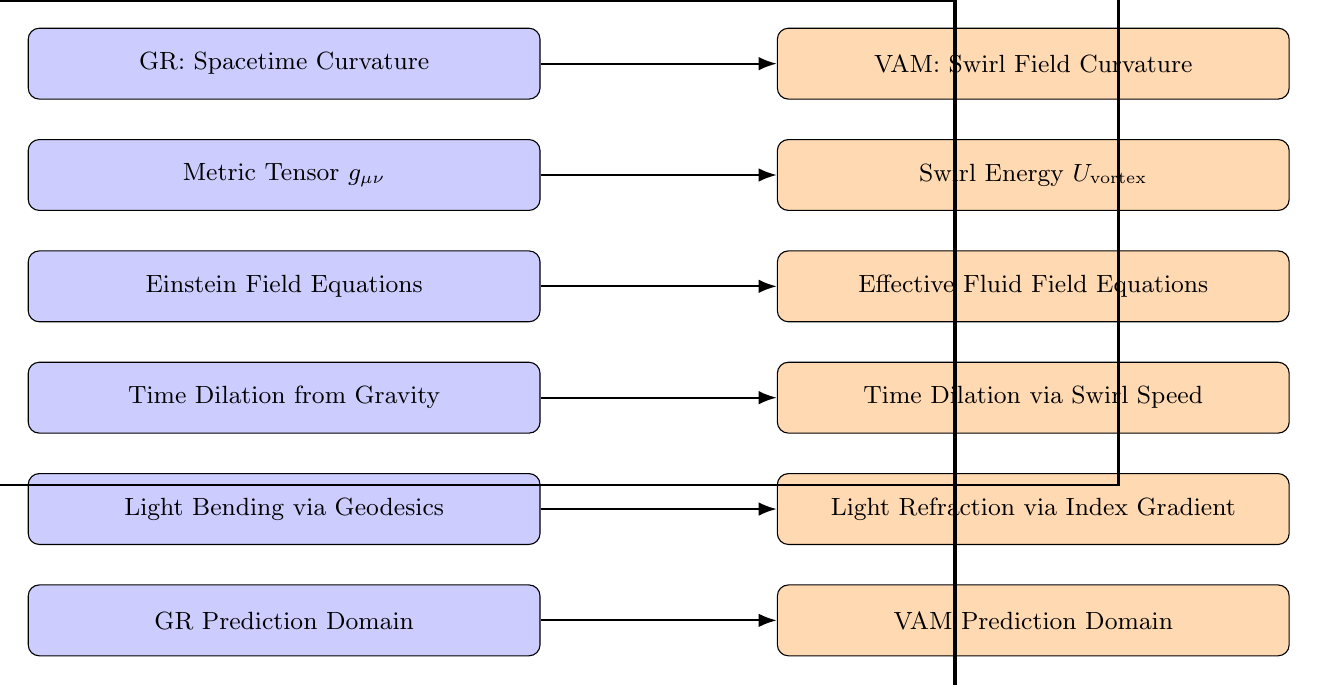
\begin{tikzpicture}[
            box/.style={rectangle, draw=black, rounded corners, minimum width=6.5cm, minimum height=0.9cm, text centered, font=\small},
            grbox/.style={box, fill=blue!20},
            vambox/.style={box, fill=orange!30},
            arrow/.style={-Latex, thick},
            node distance=0.5cm,
            every node/.append style={align=center}
        ]

            % Left GR column (aligned)
            \node[grbox] (gr1) at (-4,3.5) {GR: Spacetime Curvature};
            \node[grbox, below=of gr1] (gr2) {Metric Tensor $g_{\mu\nu}$};
            \node[grbox, below=of gr2] (gr3) {Einstein Field Equations};
            \node[grbox, below=of gr3] (gr4) {Time Dilation from Gravity};
            \node[grbox, below=of gr4] (gr5) {Light Bending via Geodesics};
            \node[grbox, below=of gr5] (gr6) {GR Prediction Domain};

            % Right VAM column
            \node[vambox, right=3cm of gr1] (vam1) {VAM: Swirl Field Curvature};
            \node[vambox, below=of vam1] (vam2) {Swirl Energy $U_{\text{vortex}}$};
            \node[vambox, below=of vam2] (vam3) {Effective Fluid Field Equations};
            \node[vambox, below=of vam3] (vam4) {Time Dilation via Swirl Speed};
            \node[vambox, below=of vam4] (vam5) {Light Refraction via Index Gradient};
            \node[vambox, below=of vam5] (vam6) {VAM Prediction Domain};


            % Horizontal arrows
            \draw[arrow] (gr1.east) -- (vam1.west);
            \draw[arrow] (gr2.east) -- (vam2.west);
            \draw[arrow] (gr3.east) -- (vam3.west);
            \draw[arrow] (gr4.east) -- (vam4.west);
            \draw[arrow] (gr5.east) -- (vam5.west);
            \draw[arrow] (gr6.east) -- (vam6.west);


        \end{tikzpicture}
        \caption{High-level correspondence between General Relativity constructs and their Vortex Æther Model analogues.}
        \label{fig:gr-vam-textmap}
    \end{figure}

% -------------------------------------------------


    \subsection*{Swirl Metric vs Spacetime Metric}

    In VAM, a local swirl-induced time element is:
    \[
        d\tau^2 = \left(1 - \frac{|\vec{v}_\theta|^2}{c^2} \right) d\mathcal{N}^2,
    \]
    where \( \vec{v}_\theta = \vec{\omega} \times \vec{r} \) is the tangential vortex velocity.

    We define an effective “swirl interval”:
    \[
        ds^2 = C_e^2 dT_v^2 - dr^2,
    \]
    analogous to the Minkowski line element, with \( C_e \) modulated by local fluid energy density. See ~\ref{sec:interpretation_c_e} for details on \( C_e \).

    We conjecture that \textbf{swirl energy curvature} replaces Ricci curvature in GR:
    \[
        \mathcal{R}_{\mu\nu}^{\text{(fluid)}} \sim \nabla_\mu \omega_\nu + \Phi_{\mu\nu}^{\text{(swirl)}},
    \]
    where \( \Phi \) encodes nonlinear swirl pressure gradients.
This echoes the Sakharov-induced gravity paradigm, where spacetime curvature emerges from microscopic degrees of freedom \cite{sakharov1967vacuum}.


    \subsection*{Effective Gravitational Redshift from Vortex Energy}

    For a particle or clock immersed in a radial vortex:
    \[
        \vec{v}_\theta(r) = \frac{\Gamma}{2\pi r} \hat{\theta}, \quad |\vec{v}_\theta|^2 \sim \frac{1}{r^2}.
    \]
    The local time flow is:
    \begin{equation}
        \boxed{
            \frac{d\tau}{d\mathcal{N}} = \sqrt{1 - \frac{\Gamma^2}{4\pi^2 r^2 c^2}}
        }
        \label{eq:gravitational-redshift}
    \end{equation}
    This mimics Schwarzschild time dilation:
    \[
        d\tau = \sqrt{1 - \frac{2GM}{rc^2}} \, dt.
    \]

    \textbf{Interpretation:} Gravitational time dilation arises from \textbf{vortex energy density}, not from spacetime curvature.

    \subsection*{Geodesic Deviation as Swirl-Advection}

    Particles follow minimal-energy paths in a curved swirl field. Define the effective swirl force:
    \[
        \vec{F}_{\text{swirl}} = -\nabla \left( \frac{1}{2} |\vec{v}_\theta|^2 \right).
    \]
    Compare to Newtonian:
    \[
        \vec{F}_g = -\nabla \Phi = -\frac{GM}{r^2} \hat{r}.
    \]
    In limit \( |\vec{v}_\theta| \propto 1/\sqrt{r} \), the effective vortex force reproduces inverse-square gravity.

    \subsection*{Light Bending and Swirl Gradient Refraction}

    In VAM, light travels as wavefronts in a medium with index \( n(x) \sim \Phi_{\text{vortex}} \). As with Fermat’s principle, curved rays emerge:
    \begin{eqbox}
        \begin{equation}
            \frac{d^{2x^i}}{ds^2} = \partial^i \log n(x)
        \end{equation}
    \end{eqbox}

    analogous to null geodesics in curved spacetime.

    \subsection*{Einstein Tensor Analogue in Fluid Field}

    Let swirl energy density \( U_{\text{vortex}} = \frac{1}{2} \rho_{\text{\ae}} |\vec{\omega}|^2 \). Then define effective Einstein tensor:
    \begin{eqbox}
        \begin{equation}
            G_{\mu\nu}^{\text{eff}} = \kappa \, T_{\mu\nu}^{\text{(vortex)}}
        \end{equation}
    \end{eqbox}

    where:
    \begin{itemize}
        \item \( T_{\mu\nu}^{\text{(vortex)}} \): momentum flux of swirl energy.
        \item \( \kappa \): coupling from æther compressibility or vortex inertia.
    \end{itemize}

    This provides an effective field equation that mirrors Einstein's:
    \[
        R_{\mu\nu} - \frac{1}{2}g_{\mu\nu}R = \kappa T_{\mu\nu}.
    \]

% -------------------------------------------------


    \subsection*{Deviations at High Vorticity}

    Where swirl speeds approach \( c \), deviations from GR predictions arise:
    \begin{itemize}
        \item Gravitational wave speed dispersion (due to fluid nonlinearity)
        \item Frame-dragging asymmetry depending on swirl chirality
        \item Breakdown of Birkhoff’s theorem: spherically symmetric fields may support residual swirl
    \end{itemize}

% -------------------------------------------------


\section*{Conclusion and Discussion:}
    \section*{Toward a Fluid Ontology of Spacetime}

    This work has demonstrated that both the kinematics of Special Relativity and the curvature-based phenomena of General Relativity can emerge from structured dynamics within a physically motivated æther. In the Vortex Æther Model (VAM), we depart from geometric axiomatics and instead reconstruct relativistic physics from first principles grounded in fluid mechanics, topological stability, and internal phase clocks.

    \subsection*{Summary of Results}

    \begin{itemize}
        \item \textbf{Lorentz Symmetry Emergence:} We showed that local time dilation, length contraction, and invariant intervals naturally arise from the swirl field kinematics of vortex structures. This led to the \textit{Lorentz Recovery Theorem}, grounding inertial relativity in vortex-induced motion.

        \item \textbf{Effective Gravity via Swirl Curvature:} Swirl energy density and pressure gradients serve as dynamical analogues of mass-energy and Ricci curvature. Through detailed correspondences (Figures~\ref{fig:gr-vam-centered} and~\ref{fig:gr-vam-textmap}), we established that gravitational redshift, lensing, and geodesics all follow from coherent vortex motion in an ætheric medium.

        \item \textbf{New Temporal Constructs:} Time in VAM is not monolithic. The model articulates a plural ontology of temporal phenomena, ranging from the universal flow of \( \mathcal{N} \), to internal phase clocks \( S(t) \), to loop-based time \( T_v \), each with distinct dynamical roles and causal implications.

        \item \textbf{Beyond Relativity:} VAM predicts observable deviations in high-vorticity regimes, where Lorentz invariance becomes approximate and topological transitions induce temporal discontinuities or quantization. This positions the model to make falsifiable predictions beyond the reach of General Relativity and Special Relativity.
    \end{itemize}

    \subsection*{Theoretical Implications}

    The Vortex Æther Model invites a radical ontological rethinking of spacetime: rather than fundamental geometric structure, spacetime emerges as a fluid epiphenomenon—cohering from rotational and topological excitations in a deeper substratum. This echoes a broader paradigm shift seen in quantum gravity research, condensed matter analogues, and emergent spacetime frameworks.

    Importantly, VAM retains objective simultaneity via the universal time coordinate \( \mathcal{N} \), offering new tools to address paradoxes in entanglement, decoherence, and temporal asymmetry without invoking geometric singularities or dark entities.

    \subsection*{Experimental Prospects}

    Several phenomena predicted by VAM are ripe for experimental interrogation:

    \begin{itemize}
        \item Anisotropic time dilation in rotational interferometry.
        \item Quantized phase discontinuities observable in precision atomic clocks or photon entanglement near vortex-rich media.
        \item Superluminal signal anomalies consistent with internal swirl coherence rather than spacetime causality violation.
    \end{itemize}

    Metamaterial analogues, superfluid systems, and acoustic black hole experiments could serve as testbeds for VAM's predictions—especially where controlled vorticity and topological excitations are feasible. Recent advances in analogue gravity systems, including quantum Hawking radiation in BECs and wave tank simulations of black hole horizons, provide feasible testbeds for VAM-like predictions \cite{steinhauer2016hawking, weinfurtner2011hawking}.

    \subsection*{Outlook}

    This study opens several future directions:

    \begin{itemize}
        \item A full tensor formulation of the swirl field and its coupling to quantum amplitudes.
        \item Mapping VAM’s topological clock dynamics to particle identity (spin, charge, etc.).
        \item Investigating possible unification with gauge field theories through vortex algebra.
    \end{itemize}

Such directions resonate with the idea of spacetime as a quantum condensate, as discussed in emergent gravity frameworks \cite{hu2005condensate}.

    Ultimately, the Vortex Æther Model does more than reinterpret relativity—it offers a coherent, testable framework wherein spacetime, gravity, and matter are no longer primary assumptions, but emergent consequences of a deeper, whirling reality.

% -------------------------------------------------



\appendix
    \section*{Appendix A: Interpretation of \( C_e \) in the Swirl Metric}\label{sec:interpretation_c_e}
    \addcontentsline{toc}{section}{Interpretation of \( C_e \) in the Swirl Metric}

    In the Vortex \AE{}ther Model (VAM), the invariant interval is defined by the swirl clock phase dynamics as:

    \[
        ds^2 = C_e^2\, dT_v^2 - dr^2,
    \]

    where:
    \begin{itemize}
        \item \( dT_v \): proper time traced along a closed vortex structure,
        \item \( dr^2 \): Euclidean spatial displacement in the æther frame,
        \item \( C_e \): vortex-core tangential velocity (a physical constant).
    \end{itemize}

    \subsection*{Physical Meaning of \( C_e \)}

    The quantity \( C_e \approx 1.0938 \times 10^6 \, \text{m/s} \) represents the characteristic tangential velocity at the core of a stable quantized vortex in the æther. It defines the internal causal dynamics of matter-like structures and is distinct from the speed of light \( c \), which governs wavefront propagation in the medium.

    \subsection*{Role in VAM Causal Structure}

    In analogy to the Minkowski spacetime interval:
    \[
        ds^2 = c^2 dt^2 - dx^2,
    \]
    where \( c \) determines the causal boundary between time-like and light-like intervals, the VAM formulation uses \( C_e \) to establish a similar structure for vortex-based causality:

    \[
        ds^2 = 0 \quad \Rightarrow \quad \text{vortex null-surface (phase horizon)}.
    \]

    This defines the limit where internal phase changes propagate through the æther at the maximum internal coherence rate.

    \subsection*{Numerical Interpretation}

    Consider a vortex clock with proper time step \( dT_v = 1 \, \text{ps} \). Then the corresponding causal pathlength is:

    \[
        C_e \cdot dT_v = (1.0938 \times 10^6)\cdot(10^{-12}) = 1.0938 \times 10^{-6} \, \text{m}.
    \]

    This provides a measurable scale for internal phase propagation — a feature not present in traditional GR, where proper time is dimensionally unscaled.

    \subsection*{Summary Table}

    \begin{center}
        \begin{tabular}{|c|c|c|}
            \hline
            \textbf{Concept} & \textbf{General Relativity} & \textbf{Vortex Æther Model} \\
            \hline
            Speed constant & \( c \) (light speed) & \( C_e \) (vortex core velocity) \\
            \hline
            Interval form & \( ds^2 = c^2 dt^2 - dr^2 \) & \( ds^2 = C_e^2 dT_v^2 - dr^2 \) \\
            \hline
            Causal surface & Light-cone & Swirl-phase cone \\
            \hline
            Clock type & External proper time & Internal vortex time \\
            \hline
        \end{tabular}
    \end{center}

    \subsection*{Conclusion}

    The swirl interval metric, with \( C_e \) as a scaling factor, encodes internal dynamics of matter structures in the æther. While \( c \) governs relativistic signaling, \( C_e \) governs \textbf{vortex coherence}, suggesting a dual structure of causality: one external and radiative, the other internal and rotational.

\section*{Appendix B: Temporal constructs in VAM}\label{sec:temporal-constructs}
    \textbf{Æther Origin}—\( \boldsymbol{\mathcal{N}} \longrightarrow \boldsymbol{\nu_0} \longrightarrow \boldsymbol{\tau} \longrightarrow \boldsymbol{S(t)^{\bm{\circlearrowleft} / \bm{\circlearrowright}}} \longrightarrow \boldsymbol{T_v} \longrightarrow \boldsymbol{\mathbb{K}} \)
    \subsection*{Glossary of Temporal Constructs in VAM}

    \begin{description}[leftmargin=2.5cm, labelwidth=2.2cm, labelsep=0.3cm, style=nextline]

        \item[\textbf{Aithēr-Time} \(\boldsymbol{\mathcal{N}}\)]%
        \textbf{(Absolute / Universal)} — The invariant background time, representing a metaphysical present throughout the æther. Serves as the ontological ground for all temporal evolution in VAM.

        \item[\textbf{Now-Point} \(\boldsymbol{\nu_0}\)]%
        \textbf{(Local Event / Temporal Slice)} — The pointlike intersection of a system’s worldline with the universal present. Defines causally relevant instants in ætheric or field interactions.

        \item[\textbf{Chronos-Time} \(\boldsymbol{\tau}\)]%
        \textbf{(Relative / Measurable)} — Proper time measured by a moving system with respect to the æther rest frame. This corresponds to the relativistic concept of local time and appears in dilation formulas.

        \item[\textbf{Swirl Clock} \( \boldsymbol{S(t)^{\bm{\circlearrowleft} / \bm{\circlearrowright}}}\)]%
        \textbf{(Local / Cyclical)} — Internal clock-like phase variable of a vortex knot. Encodes rotation, chirality, and phase identity through time, allowing topological tracking and evolution.

        \item[\textbf{Vortex Proper Time} \(\boldsymbol{T_v}\)]%
        \textbf{(Derived / Topological)} — Time accrued along a closed-loop vortex, defined via internal phase velocity. Reflects intrinsic temporal periodicity arising from knot geometry.

        \item[\textbf{Kairos Moment} \(\boldsymbol{\mathbb{K}}\)]%
        \textbf{(Threshold / Emergent)} — Critical point where internal dynamics or external alignment produce transformation. Can signal bifurcations, phase jumps, or topological transitions.

        \item[\textbf{Æther Frame} \(\boldsymbol{\Xi_0}\)]%
        \textbf{(Reference Frame)} — Preferred global rest frame of the æther. Distinguishes inertial dynamics from swirl-induced motion and defines global synchronization relative to \(\mathcal{N}\).

    \end{description}


    Unlike relational time models in canonical quantum gravity \cite{rovelli2004quantum}, VAM retains absolute time $\mathcal{N}$ as a physically grounded backdrop.

    \bibliography{../references}
    \bibliographystyle{unsrt}

\end{document}